\chapter{Diagramas BPMN}\label{chap:bpmn-appendix}

\section{Introdução}

Os diagramas de Modelo e Notação de Processos de Negócio (Business Process Model and Notation - BPMN) servem para modelar um processo de negócio de maneira a unificar a visão sobre aquele processo e encontrar possíveis otimizações para o mesmo processo.

Para o trabalho em questão, foram usados os diagramas para levantar o processo antes do sistema, assim evidenciamos os pontos onde o sistema pode agir.

Para este projeto, foi usada a ferramenta Draw.io\cite{drawio}, para elaborar os diagramas BPMN dos processos citados. Apesar de não ser uma ferramenta específica para esse tipo de diagrama, é uma ferramenta de diagramação simples e que possui bibliotecas de diversos tipos de diagramas, inclusive os de BPMN.

\section{Processo antes do Sistema}

Os diagramas BPMN foram gerados com base nas entrevistas realizadas durante o processo de levantamento de requisitos. Vale lembrar que eles foram divididos de maneira a facilitar a visualização neste documento.

\subsection{TCC 1}
\begin{figure}[H]
    \centering
    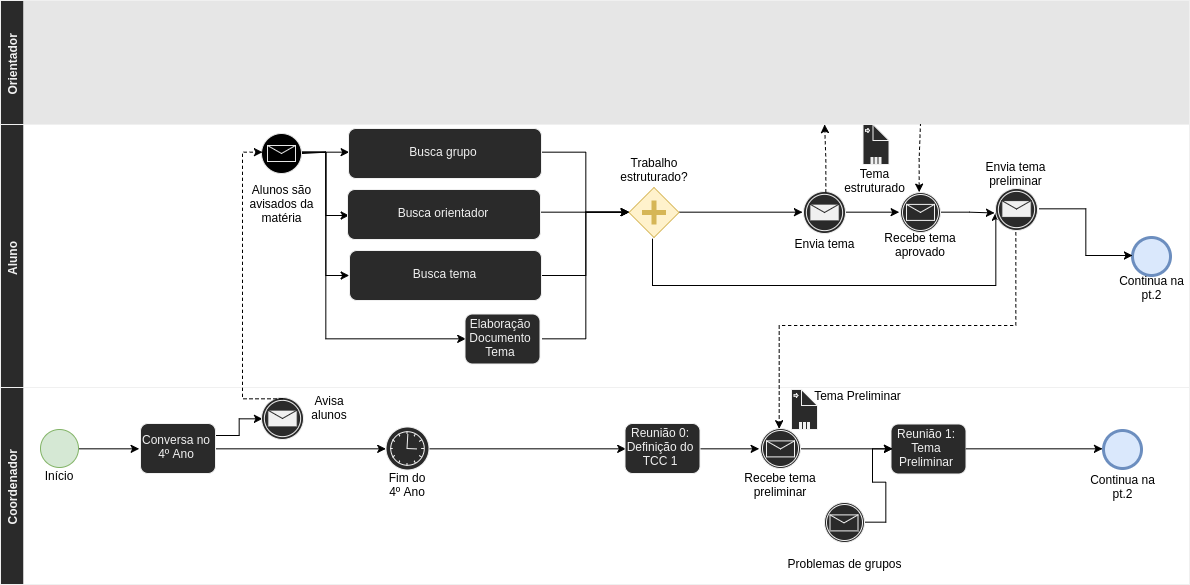
\includegraphics[angle=90, origin=c, scale=0.50]{bpmn-tcc1-pt1.png}
    \caption{Diagrama BPMN para a disciplina de TCC 1 - Parte 1}
    \label{fig:bpmn-tcc1-pt1}
\end{figure}

\begin{figure}[H]
    \centering
    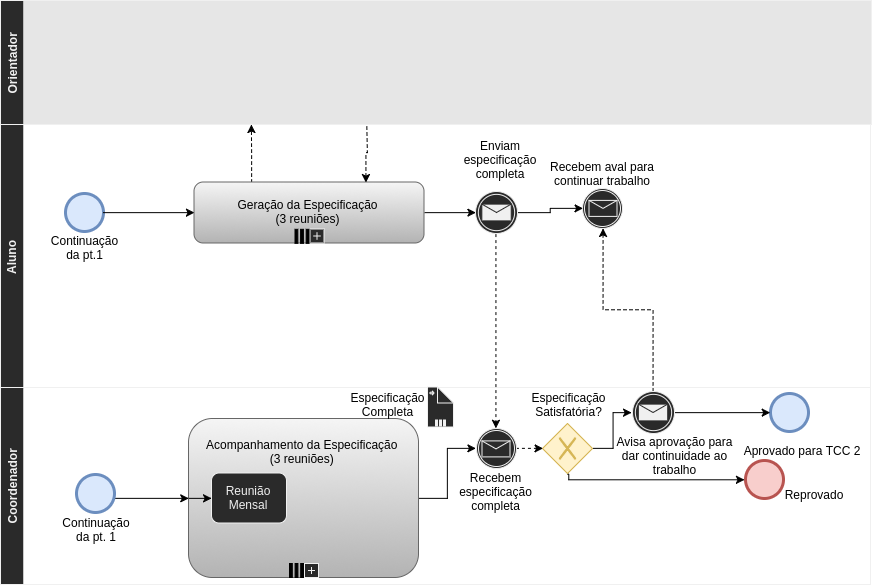
\includegraphics[angle=90, origin=c, scale=0.70]{bpmn-tcc1-pt2.png}
    \caption{Diagrama BPMN para a disciplina de TCC 1 - Parte 2}
    \label{fig:bpmn-tcc1-pt2}
\end{figure}

\subsection{TCC 2 - Sem eventos finais}
\begin{figure}[H]
    \centering
    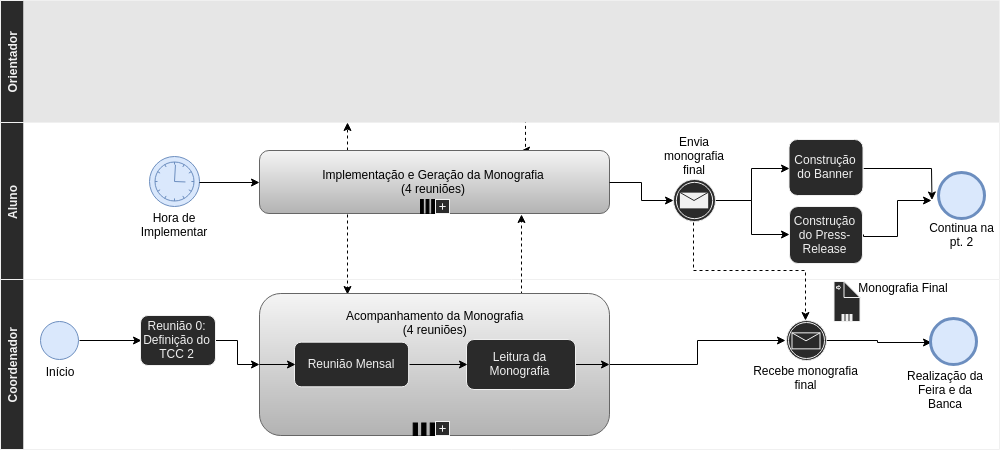
\includegraphics[angle=90, origin=c, scale=0.60]{bpmn-tcc2-pt1.png}
    \caption{Diagrama BPMN para a disciplina de TCC 2 - Parte 1}
    \label{fig:bpmn-tcc2-pt1}
\end{figure}

\begin{figure}[H]
    \centering
    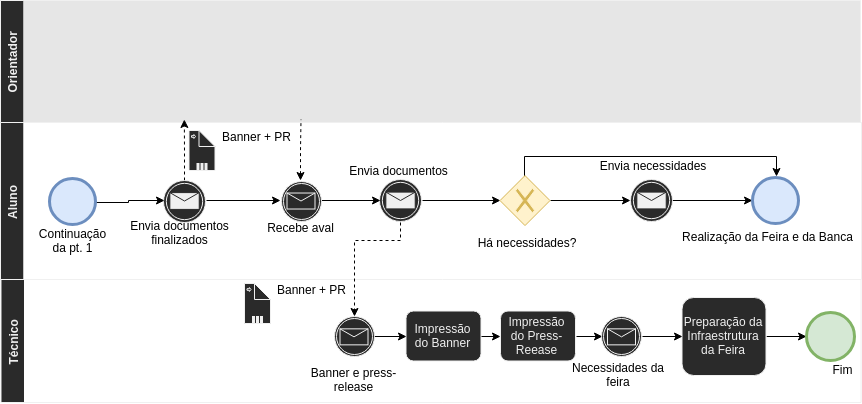
\includegraphics[angle=90, origin=c, scale=0.70]{bpmn-tcc2-pt2.png}
    \caption{Diagrama BPMN para a disciplina de TCC 2 - Parte 2}
    \label{fig:bpmn-tcc2-pt2}
\end{figure}

\subsection{Banca e Feira}
\begin{figure}[H]
    \centering
    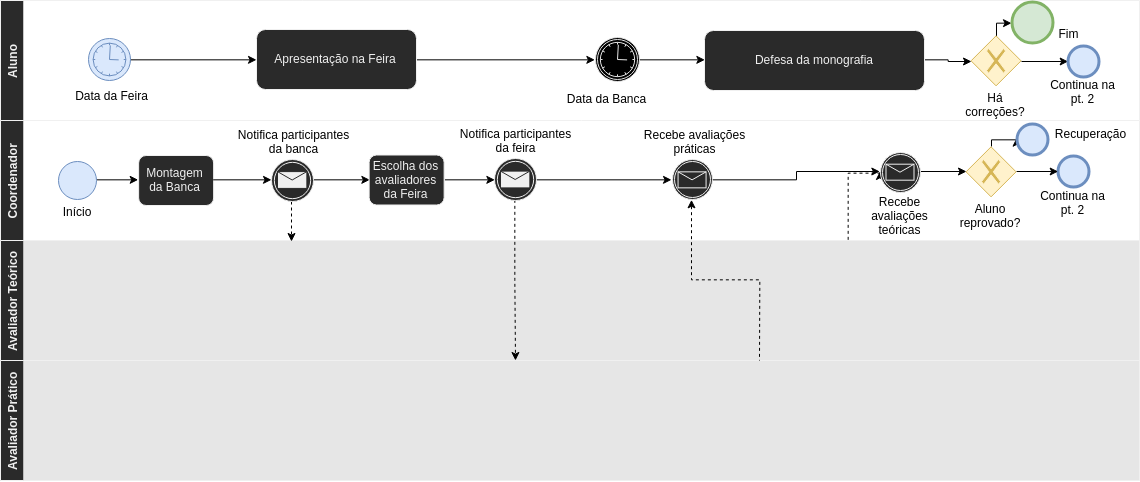
\includegraphics[angle=90, origin=c, scale=0.55]{bpmn-banca-feira-pt1.png}
    \caption{Diagrama BPMN para a Banca e Feira - Parte 1}
    \label{fig:bpmn-banca-feira-pt1}
\end{figure}

\begin{figure}[H]
    \centering
    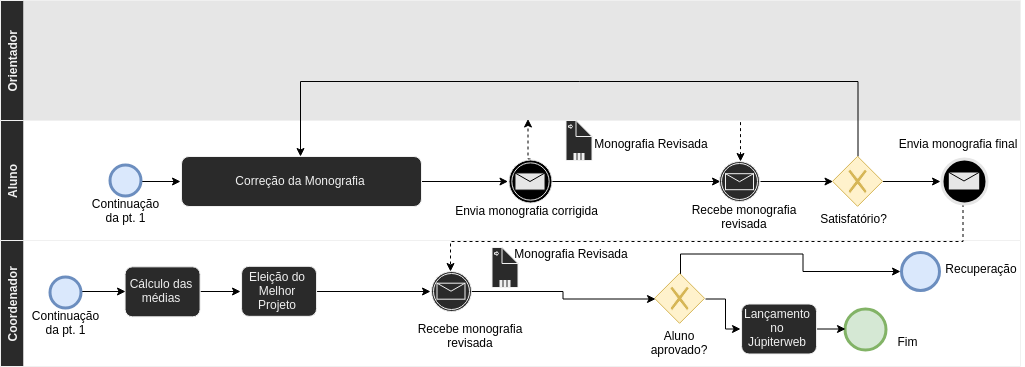
\includegraphics[angle=90, origin=c, scale=0.60]{bpmn-banca-feira-pt2.png}
    \caption{Diagrama BPMN para a Banca e Feira - Parte 2}
    \label{fig:bpmn-banca-feira-pt2}
\end{figure}

\subsection{Recuperação}
\begin{figure}[H]
    \centering
    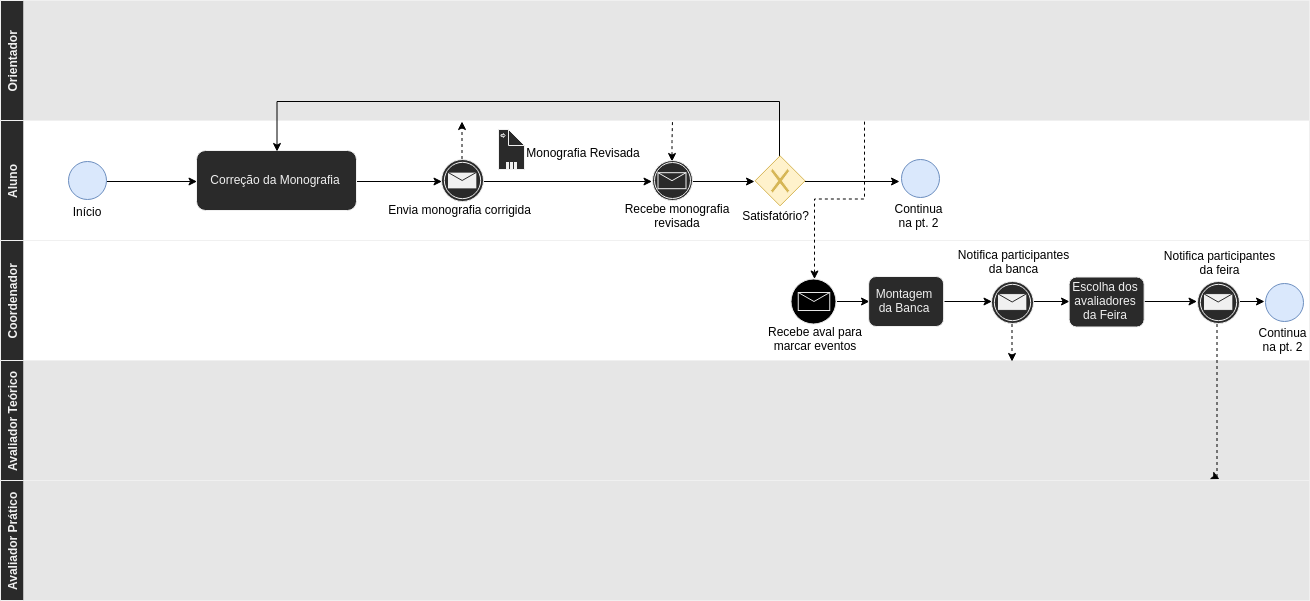
\includegraphics[angle=90, origin=c, scale=0.45]{bpmn-rec-pt1.png}
    \caption{Diagrama BPMN para a Recuperação - Parte 1}
    \label{fig:bpmn-rec-pt1}
\end{figure}

\begin{figure}[H]
    \centering
    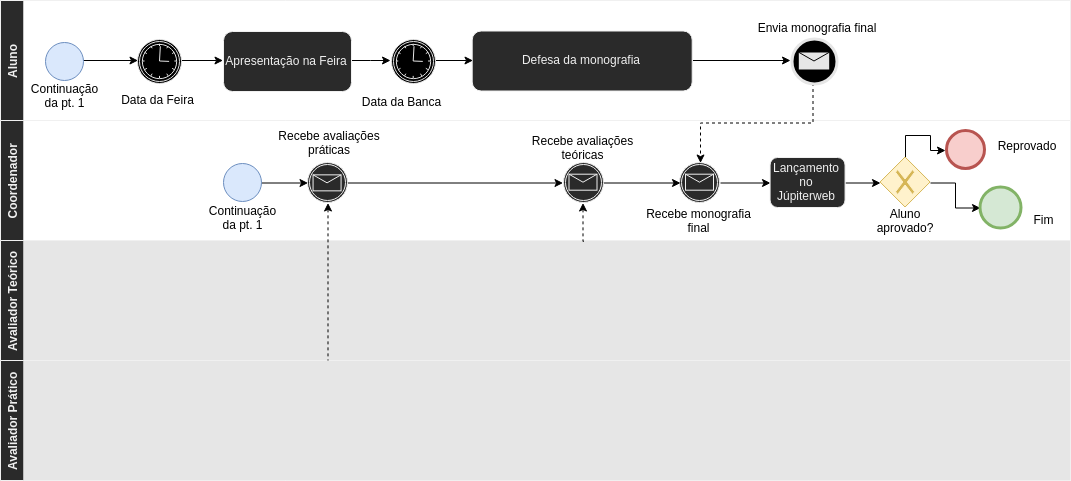
\includegraphics[angle=90, origin=c, scale=0.60]{bpmn-rec-pt2.png}
    \caption{Diagrama BPMN para a Recuperação - Parte 2}
    \label{fig:bpmn-rec-pt2}
\end{figure}
